
%
%
%

\begin{frame}[t]{The perceptron as a computational unit}

    The function computed by the \index{perceptron}\gls{perceptron},
    as well as the learning process, is similar to that of several
    other types of \index{linear model}\glspl{linear model} in \gls{ml}.
    
    The \gls{perceptron} can be seen as a {\bf computational unit}.
    
    We can combine multiple units and create more powerful models.
    
    \begin{center}
        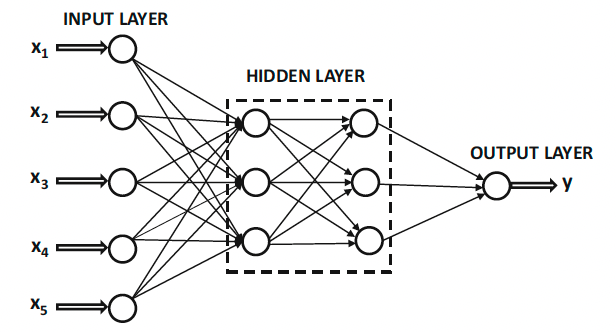
\includegraphics[width=0.70\textwidth]{./images/perceptron/combining_units.png}\\
        {\scriptsize \color{col:attribution} 
        Image reproduced from p.18 of \cite{Aggarwal:2018SpringerDL}}\\
     \end{center}
    
    
\end{frame}
